\chapter{Konzept}
\label{ch:chapter04}
In diesem Kapitel wird darauf eingegangen wie Vorgegangen wurde, um verschiedene Konzepte zu entwickeln.
Dabei werden die vorher erwähnten Befragungen (\ref{ch:Recherche}) verwendet, um eine Lösung für die individuellen Probleme zu entwickeln.
Zudem wird betrachtet der Stand der Technik betrachtet sowie einen Vergleich mit den Datenbankstrukturen gezogen.
Dies wird getan, da diese eine ähnliche Struktur wie die Profile und Berechtigungen.
Anschließend werden die Probleme aus den Befragungen quantifiziert, um daraus dann die verschiedenen Konzepte zu entwickeln.


\section{Konzeptentwicklung}
\label{sec:chapter04:Konzeptentwicklung}

\subsection{Stand der Technik}
\label{sec:chapter04:Stand}
In der Welt von Cloud Computing wird \ac{IAM} als Sicherheitsmaßnahme verwendet.
Dabei wird mittels \ac{IAM} die Identität und der Zugriff reguliert.
\ac{IAM} kann daher in die folgende fünf Punkte gegliedert werden.
\newline
\newline
1. Authentifizierung der Person
\newline
Dabei überprüft, ob die Person auch wirklich, die ist als welche diese sich ausgibt.
Hierfür gibt es verschiedene Methoden, um dies sicherzustellen.
Nutzername mit ein Passwort ist die gängigste Methoden, um dies zu tun, welche von den meisten Webseiten und Computern verwendet wird.
Um die Authentifizierung sicherer zu gestalten werden mehrere Faktoren berücksichtigt, um eine Person zu identifizieren.
Dies kann zum Beispiel durch einen Fingerabdruck stattfinden. \cite{IamIEEE} (S.1482)
\newline
\newline
2. Berechtigungsvergabe
\newline
Es beschäftigt sich damit, welche Berechtigungen der Nutzer bekommt.
Dies wird mittels Autorisierungsrichtlinien gesichert, damit die Nutzer nur Zugriff auf die Ressourcen und Dienste haben, welche diese benötigen.
Das wird mit hilfe von Profilen erreicht, welche von der Organisation zugewissen werden. \cite{IamIEEE} (S.1482)
\newline
\newline
3. Identitätsvergabe
\newline
Identitätsvergabe sorgt dafür, dass der Nutzer eine digitale ID oder Account erhält.
Wenn ein Mitarbeiter bei einem Unternehmen arbeit, erhält dieser eine digitale Identität, um auf die Ressourcen des Unternehmen zu greifen zu können.
Dabei ist auch wichtig, dass der Mitarbeiter diese digitale Identität wieder verliert, wenn dieser das Unternehmen verlässt oder an einer anderen Stelle im Unternehmen arbeitet und nicht mehr seine alte digitale Identität benötigt.
\newline
\newline
4. Föderierte Identität
\newline
Dabei handelt es sich darum, dass die digitalen Identitäten über verschiedene Anwendungen und Organisationen gültig sind.
Dadurch werden die Informationen der digitalen Identität gespeichert.
Dies hat den Vorteil, dass der Nutzer sich nur einmal anmelden muss, um auf sämtliche seiner Ressourcen zugreifen zu können.
Dabei werden Protokolle wie SAML, OAuth oder OpenID verwendet.
Die Folge dadurch ist, dass der Nutzer sich nicht mehrere Passwörter sowie Accounts merken muss. \cite{IamIEEE} (S.1482)
\newline
\newline
5. Compliance Verwaltung
\newline
Die Compliance Verwaltung überprüft die Authentifizierung- und Zugriffaufzeichnungen, um sicher zustellen, dass die Richlinien und Sicherheitsstandards eingehalten wurden.
Diese Überprüfung ist notwendig für effektive Zugriffregeln.
Zudem werden diese für Audits benötigt. \cite{IamIEEE} (S.1482)
\newline
\newline
\begin{figure}[h!]
 \centering
 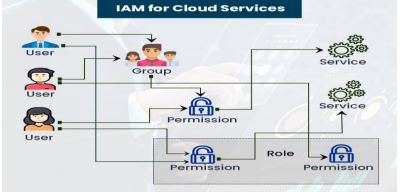
\includegraphics[width=1\textwidth]{gfx/Picture/IAMISH.PNG}
 \caption{IAM für Cloud Dienste \cite{Moha19} (Seite 3)}
 \label{fig:IMAISH}
\end{figure}
Dies ist ein Beispiel wie die oben genannten Punkte umgesetzt werden können.
Dabei haben die Accounts der Personen entweder direkte Berechtigung oder diese werden mittels Gruppen verteilt.
Sobald der Account die Berechtigung hat, kann dieser auf die dahinter steckende Ressource zugreifen.
Die Berechtigungen können dabei auch mittels Profile zusammengefasst werden.
\newline
Dabei kann dies auch verschiedenen Wegen umgesetzt werden, da die selbe Lösung für gewisse Fälle nicht funktioniert.
Zum Beispiel die Quelle \cite{Cal17}(S.208) beschreibt das Problem wie die United States of America am besten mit ihren Verbündeten kooperieren soll.
Da es dabei um sensitive Informationen handelt, welche an verschiedenen Partnern vermittelt werden, muss der Zugriff reguliert werden.
Besonders haben die verschiedenen Ländern verschiedene Gesetzte, worauf auch geachtet werden muss. 
Deswegen gibt es nicht die eine Lösung, um die Herausforderung zu lösen. \cite{Cal17} (S.208)


\subsection{Vergleich mit Datenbanken}
\label{sec:chapter04:DB}
Die Helvetia verwendet zum Speichern der Informationen für die Berechtigungsstruktur so genannte HV-Tabellen.
Bei diesen HV-Tabellen handelt es sich dabei, um DB2-Tabellen.
Deswegen wird betrachtet, wie der Standard mit Account innerhalb von Datenbanken ist.
\newline
Berechtigungen für Rollen wird mittels GRANT...ON...TO...[GRANT OPTION] vergeben.
Dabei wird die spezifische Berechtigungen, zum Beispiel eine View und Account oder Gruppen angegeben.
Zudem kann auch hinzugefügt werden, ob die Rolle die Berechtigung hat anderen Accounts die Berechtigungen zu geben.\cite{Ram09} (S.474-475)
\newline
Wenn man sich zum Beispiel das Bild (\ref{fig:Berch}) ansieht könnte zum Beispiel der Befehl wie folgt aussehen:
\newline
\newline
GRANT UPDATE ON PKU00 TO L895.
\newline
\newline
Das würde zum Beispiel bedeuten, dass der Nutzer L895 die Bearbeitungsberechtigung für die Ressource PKU00 erhalten hat.
Dabei kommt auch die Frage, was man eher verwenden sollte.
Indviduelle Berechtigungsvergabe oder über Gruppenvergabe für die Accounts.
Microsoft hat folgendes als Best Practise definiert:
\newline
\newline
\textit{"`To simplify administration, create groups and assign each group permission to functional areas and model objects.
You can then add and remove users from the groups without accessing the Master Data Manager UI.
\newline
\newline
Do not assign additional permissions to an individual user, and do not include a user in multiple groups that have access to Master Data Manager. In addition, do not use hierarchy member permissions unless you want a group to have limited access to specific members."'} \cite{Micro}
\newline
\newline
Micrsoft gibt an, dass man Gruppen erstellen, die individuellen Nutzer keine zusätzlichen Berechtigungen bekommen sollen und nicht in mehreren Gruppen sein soll, die Zugriff auf den Master Data Manager haben.
IBM gibt eine ähnlich Best Practise an, dass Angestellte in einem Unternehmen mittels Gruppen organisiert werden sollten. \cite{IBMGroup}

\section{Herausforderung}
\label{sec:chapter04:Herausforderung}
Sed lobortis vestibulum euismod. Vivamus vestibulum gravida nisi vitae condimentum. Nullam nec lacus nibh. Phasellus arcu magna, varius eget viverra a, elementum eu dolor. Aliquam erat volutpat. Sed nibh leo, vestibulum quis lacinia in, vestibulum sollicitudin nulla. In iaculis, purus in imperdiet sagittis, tortor diam pellentesque lectus, eget faucibus ante elit at tortor.

\section{Konzept A}
\label{sec:chapter03:tabellen}
Sed lobortis vestibulum euismod. Vivamus vestibulum gravida nisi vitae condimentum. Nullam nec lacus nibh. Phasellus arcu magna, varius eget viverra a, elementum eu dolor. Aliquam erat volutpat. Sed nibh leo, vestibulum quis lacinia in, vestibulum sollicitudin nulla. In iaculis, purus in imperdiet sagittis, tortor diam pellentesque lectus, eget faucibus ante elit at tortor.


\section{Konzept B}
\label{sec:chapter04:minimal}
Aliquam ut pretium lectus. Curabitur in eros et sapien aliquet luctus ut sit amet eros. Proin et libero non mi venenatis aliquet at sed lorem. Ut sed enim mi, id viverra eros. Cras metus ante, placerat id commodo at, molestie non libero. Aenean eu risus erat, vel consequat metus. Sed malesuada metus sit amet nisl viverra hendrerit.


